\documentclass[aspectratio=169, 10pt]{beamer}

% ==============================================================================
% GÓI VÀ CẤU HÌNH GIAO DIỆN BEAMER
% ==============================================================================
\usepackage[utf8]{inputenc}
\usepackage[vietnamese,english]{babel}
\usepackage[T5]{fontenc}
\usepackage{lmodern}
\usepackage{amsmath,amssymb}
\usepackage{booktabs}
\usepackage{tabularx}
\usepackage{graphicx}
\usepackage{xcolor}
\usepackage{colortbl}
\usepackage{tikz}

% Chủ đề Beamer thanh lịch, học thuật
\usetheme{Madrid}
\usecolortheme{whale}

% Định nghĩa bảng màu nhận diện ĐH Bách Khoa
\definecolor{bkblue}{RGB}{13, 71, 161}      % Xanh dương đậm HCMUT
\definecolor{bkcyan}{RGB}{0, 172, 193}      % Xanh ngọc
\definecolor{bkgray}{RGB}{245, 247, 250}    % Xám nền nhẹ
\definecolor{darkred}{RGB}{183, 28, 28}     % Đỏ cảnh báo / Failure mode
\definecolor{darkgreen}{RGB}{46, 125, 50}   % Xanh lá thành công

\setbeamercolor{palette primary}{bg=bkblue,fg=white}
\setbeamercolor{palette secondary}{bg=bkblue!85!black,fg=white}
\setbeamercolor{palette tertiary}{bg=bkblue!70!black,fg=white}
\setbeamercolor{structure}{fg=bkblue}
\setbeamercolor{titlelike}{parent=palette primary}
\setbeamercolor{block title}{bg=bkblue,fg=white}
\setbeamercolor{block body}{bg=bkgray,fg=black}
\setbeamercolor{block title alerted}{bg=darkred,fg=white}
\setbeamercolor{block body alerted}{bg=darkred!8,fg=black}
\setbeamercolor{block title example}{bg=darkgreen,fg=white}
\setbeamercolor{block body example}{bg=darkgreen!8,fg=black}

\setbeamertemplate{navigation symbols}{}
\setbeamertemplate{caption}[numbered]

% ==============================================================================
% THÔNG TIN TIÊU ĐỀ
% ==============================================================================
\title[CO3133 -- Báo Cáo Tiến Độ Số 3]{Phát Triển Hệ Thống Phân Đoạn Thực Thể và Định Vị 3D Mục Tiêu Sầu Riêng Dựa Trên YOLOv8-Seg và Cảm Biến Độ Sâu cho Robot Nông Nghiệp Tự Hành}
\subtitle{Báo Cáo Tiến Độ Số 03 (Sprint 3: 12/10 -- 25/10/2026) \textbar\ Học Kỳ Doanh Nghiệp HK261}

\author[Trần Hữu Hoàng Long \& Trương Gia Hy]{
    \textbf{Sinh viên thực hiện:}\\
    Trần Hữu Hoàng Long (MSSV: 2352704) \quad\textbar\quad Trương Gia Hy (MSSV: 2352458)\\[4pt]
    \textbf{Giảng viên hướng dẫn:} ThS. Nguyễn Quốc Minh
}

\institute[HCMUT -- CSE]{
    Khoa Khoa học và Kỹ thuật Máy tính -- Trường Đại học Bách khoa, ĐHQG-HCM\\[2pt]
    Môn học: \textbf{Học sâu và Ứng dụng (CO3133)} \textbar\ Đề án Doanh nghiệp gốc: \textbf{HK261-DAGD1-558}
}

\date[25/10/2026]{TP. Hồ Chí Minh, Ngày 25 Tháng 10 Năm 2026}

\logo{\IfFileExists{HCMUT-logo.png}{
\includegraphics[height=0.7cm]{HCMUT-logo.png}}{}}

% ==============================================================================
% BẮT ĐẦU NỘI DUNG SLIDE
% ==============================================================================
\begin{document}
\selectlanguage{vietnamese}

% ------------------------------------------------------------------------------
% SLIDE 1: TRANG TIÊU ĐỀ
% ------------------------------------------------------------------------------
\begin{frame}
    \titlepage
\end{frame}

% ------------------------------------------------------------------------------
% SLIDE 2: TỔNG KẾT ÁNH XẠ CHUẨN ĐẦU RA (CĐR)
% ------------------------------------------------------------------------------
\begin{frame}{Chuẩn đầu ra môn học CO3133 (Course Learning Outcomes)}
\footnotesize
Báo cáo và bài thuyết trình đáp ứng đầy đủ 4 Chuẩn đầu ra cốt lõi của đề cương môn học:
\vspace{0.15cm}
\begin{table}[htbp]
\centering
\scriptsize
\renewcommand{\arraystretch}{1.1}
\begin{tabularx}{\textwidth}{l p{4.2cm} X c}
\toprule
\textbf{Chuẩn đầu ra} & \textbf{Nội dung học phần} & \textbf{Minh chứng kỹ thuật trong Báo cáo 3} & \textbf{Trạng thái} \\
\midrule
\textbf{CĐR 8 (L.O.5.1)} & Đánh giá mô hình học sâu qua ablation, loss curve, error analysis. & Benchmark 5 kịch bản trên RTX 3060, phân tích cú nảy gradient ngắt Mosaic, tính Wilson 95\% CI cho Recall. & \textbf{Hoàn thành} \\
\textbf{CĐR 9 (L.O.5.2)} & Phân tích đánh đổi kỹ thuật (accuracy, latency, RAM, nhiệt độ) trên kit nhúng. & Đánh đổi Nano vs Small, ngân sách CPU/RAM trên Raspberry Pi 5 16GB, phân tích ca lỗi OOD thực tế. & \textbf{Hoàn thành} \\
\textbf{CĐR 4 (L.O.4.1)} & Hiện thực, huấn luyện mô hình học sâu trên trạm GPU chuyên dụng. & Huấn luyện PyTorch 2.3.0, Ultralytics 8.2 trên GPU NVIDIA RTX 3060 (12\,GB VRAM). & \textbf{Hoàn thành} \\
\textbf{CĐR 5 (L.O.4.2)} & Thu thập, chuẩn hóa, chống rò rỉ và tăng cường dữ liệu. & Gộp 5 kho Roboflow (2,676 ảnh), chuẩn hóa tọa độ nhãn [0, 1], tăng cường trực tuyến (online GPU). & \textbf{Hoàn thành} \\
\bottomrule
\end{tabularx}
\end{table}
\end{frame}

% ------------------------------------------------------------------------------
% SLIDE 3: BỐI CẢNH DỰ ÁN & MỤC TIÊU UGV
% ------------------------------------------------------------------------------
\begin{frame}{Bối cảnh Dự án \& Mục tiêu Kỹ thuật (Project Kickoff)}
\begin{columns}[T]
\begin{column}{0.48\textwidth}
    \begin{block}{Bài toán Nông nghiệp Đồi dốc}
    \footnotesize
    \begin{itemize}
        \item Cây sầu riêng (*Durio zibethinus*) mẫn cảm với bệnh xì mủ thối quả do nấm *Phytophthora*.
        \item Phun thuốc thủ công trên sườn đồi dốc hiểm trở gây độc hại, lãng phí 60--70\% hóa chất.
        \item \textbf{Đề án HK261-DAGD1-558:} Phát triển robot UGV tự hành gắn tháp pháo phun thuốc 2 trục (pan-tilt).
    \end{itemize}
    \end{block}
\end{column}
\begin{column}{0.48\textwidth}
    \begin{block}{Nhiệm vụ Phân hệ Thị giác Máy tính}
    \footnotesize
    \begin{itemize}
        \item Nhận diện chính xác từng quả sầu riêng đang treo trên tán lá cây từ camera RGB-D.
        \item Trích xuất tọa độ không gian 3D $(X, Y, Z)$ thời gian thực để dẫn động vòi phun ngắm bắn tâm quả.
        \item \textbf{Ràng buộc thực tế:} Phải chạy ổn định trên phần cứng nhúng UGV (\textbf{Raspberry Pi 5 16GB}, camera \textbf{RealSense D453i}, \textbf{LiDAR C1M1}).
    \end{itemize}
    \end{block}
\end{column}
\end{columns}
\end{frame}

% ------------------------------------------------------------------------------
% SLIDE 4: CƠ SỞ KHOA HỌC: BBOX 2D VS INSTANCE SEGMENTATION
% ------------------------------------------------------------------------------
\begin{frame}{Cơ sở Khoa học: Hộp bao 2D vs. Phân đoạn Thực thể}
\begin{columns}[T]
\begin{column}{0.48\textwidth}
    \begin{alertblock}{Hạn chế của Hộp bao chữ nhật 2D}
    \footnotesize
    \begin{itemize}
        \item Hộp bao chữ nhật ôm trùm cả khoảng trống kẽ lá và cành cây (chiếm 20--40\% diện tích).
        \item \textbf{Lỗi Depth Bleeding:} 
        \begin{itemize}
            \scriptsize
            \item Tâm hộp bao rơi vào kẽ lá $\rightarrow$ đo nhầm độ sâu của hậu cảnh xa ($Z_{\text{đo}} \gg Z_{\text{quả}}$).
            \item Có lá chắn trước quả $\rightarrow$ đo nhầm độ sâu của tiền cảnh gần ($Z_{\text{đo}} < Z_{\text{quả}}$).
        \end{itemize}
        \item Hậu quả: Tháp pháo tính sai cự ly ngắm bắn, phun trượt quả!
    \end{itemize}
    \end{alertblock}
\end{column}
\begin{column}{0.48\textwidth}
    \begin{exampleblock}{Cơ sở từ Y văn Quốc tế (Literature)}
    \footnotesize
    \begin{itemize}
        \item \textbf{Fu et al. (2020) \cite{fu2020rgbd}} (\textit{Comput. Electron. Agric.}): Tổng quan chứng minh việc lấy mẫu depth qua tâm BBox luôn bị sai số lớn do kẽ lá và che khuất.
        \item \textbf{Lin et al. (2021) \cite{lin2021fruit}} \& \textbf{Kang \& Chen (2020) \cite{kang2020dasnet}}: Mặt nạ phân đoạn thực thể bóc tách chính xác viền quả, đưa sai số 3D về cấp milimet.
        \item $\rightarrow$ \textbf{Lựa chọn:} Dùng \textbf{YOLOv8-Seg} để tạo mặt nạ pixel lọc sạch điểm ảnh nền.
    \end{itemize}
    \end{exampleblock}
\end{column}
\end{columns}
\end{frame}

% ------------------------------------------------------------------------------
% SLIDE 5: DỮ LIỆU & TĂNG CƯỜNG TRỰC TUYẾN
% ------------------------------------------------------------------------------
\begin{frame}{Chuẩn Hóa Dữ Liệu \& Tăng Cường Trực Tuyến (Trọng tâm CĐR 5)}
\begin{columns}[T]
\begin{column}{0.48\textwidth}
    \begin{block}{Hợp nhất 5 Kho Dữ liệu (2,676 ảnh)}
    \footnotesize
    \begin{itemize}
        \item Nguồn: 5 tập dữ liệu Roboflow mở (giống Udang Merah, Puyat, vườn hỗn hợp, ảnh rãnh gai).
        \item Đồng nhất tất cả về 1 lớp nhãn: \texttt{durian} (ID 0).
        \item \textbf{Chuẩn hóa tọa độ [0, 1]:} Chia tọa độ pixel $(x, y)$ cho $(W, H)$ theo chuẩn YOLOv8 để mạng thích ứng đa tỷ lệ.
        \item Phân chia độc lập: \textbf{Train 80\%} (2,129 ảnh), \textbf{Val 14\%} (379 ảnh), \textbf{Test 6\%} (168 ảnh).
    \end{itemize}
    \end{block}
\end{column}
\begin{column}{0.48\textwidth}
    \begin{alertblock}{Cơ chế Online Augmentation (GPU VRAM)}
    \footnotesize
    \begin{itemize}
        \item Biến đổi ngẫu nhiên từng batch trực tiếp trong bộ nhớ GPU: Mosaic, HSV jitter, lật ngang, co giãn.
        \item Không sinh ảnh tĩnh trùng lặp trên ổ cứng.
        \item Tập Val và Test giữ nguyên bản tuyệt đối để kiểm định trung thực.
    \end{itemize}
    \end{alertblock}
\end{column}
\end{columns}
\end{frame}

% ------------------------------------------------------------------------------
% SLIDE 6: 4 HÀM MẤT MÁT MẶC ĐỊNH CỦA YOLOV8-SEG
% ------------------------------------------------------------------------------
\begin{frame}{4 Hàm Mất Mát Mặc Định của Kiến Trúc YOLOv8-Seg}
\footnotesize
YOLOv8-Seg tối ưu hóa đồng thời 4 thành phần mất mát mặc định do Ultralytics thiết kế:
\begin{equation*}
\mathcal{L}_{\text{total}} = 7.5\,\mathcal{L}_{\text{CIoU}} + 1.5\,\mathcal{L}_{\text{DFL}} + 0.5\,\mathcal{L}_{\text{BCE\_cls}} + 2.5\,\mathcal{L}_{\text{BCE\_mask}}
\end{equation*}

\begin{columns}[T]
\begin{column}{0.48\textwidth}
    \begin{block}{Complete IoU Loss ($\mathcal{L}_{\text{CIoU}}$) \cite{zheng2020ciou}}
    \scriptsize
    Tối ưu đồng thời độ trùng khớp diện tích, khoảng cách tâm chuẩn hóa và tính nhất quán tỷ lệ khung hình:
    $$\mathcal{L}_{\text{CIoU}} = 1 - \text{IoU} + \frac{\rho^2(\mathbf{b}, \mathbf{b}^{gt})}{c^2} + \alpha v$$
    \end{block}
    \begin{block}{Distribution Focal Loss ($\mathcal{L}_{\text{DFL}}$) \cite{li2020generalized}}
    \scriptsize
    Mô hình hóa tọa độ hộp bao thành phân phối xác suất rời rạc, nắm bắt độ bất định tại các rãnh gai gồ ghề.
    \end{block}
\end{column}
\begin{column}{0.48\textwidth}
    \begin{block}{Classification Loss ($\mathcal{L}_{\text{BCE\_cls}}$)}
    \scriptsize
    Mất mát Binary Cross-Entropy trên logit dự đoán xác suất lớp \texttt{durian}.
    \end{block}
    \begin{block}{Mask Loss ($\mathcal{L}_{\text{BCE\_mask}}$)}
    \scriptsize
    Mất mát BCE cấp điểm ảnh giữa nhãn ground-truth và mặt nạ tái tạo từ tổ hợp 32 prototype masks của nhánh ProtoNet:
    $$\hat{M}(u, v) = \sigma\left(\sum_{k=1}^{32} w_k P_k(u, v)\right)$$
    \end{block}
\end{column}
\end{columns}
\end{frame}

% ------------------------------------------------------------------------------
% SLIDE 7: HỘI TỤ VÀ NGẮT MOSAIC TẠI EPOCH 20
% ------------------------------------------------------------------------------
\begin{frame}{Động Lực Học Hội Tụ \& Ngắt Mosaic ở 10 Epoch Cuối}
\begin{columns}[c]
\begin{column}{0.52\textwidth}
    \centering
    \IfFileExists{baseline_yolov8n_640_b16_e30_results.png}{
        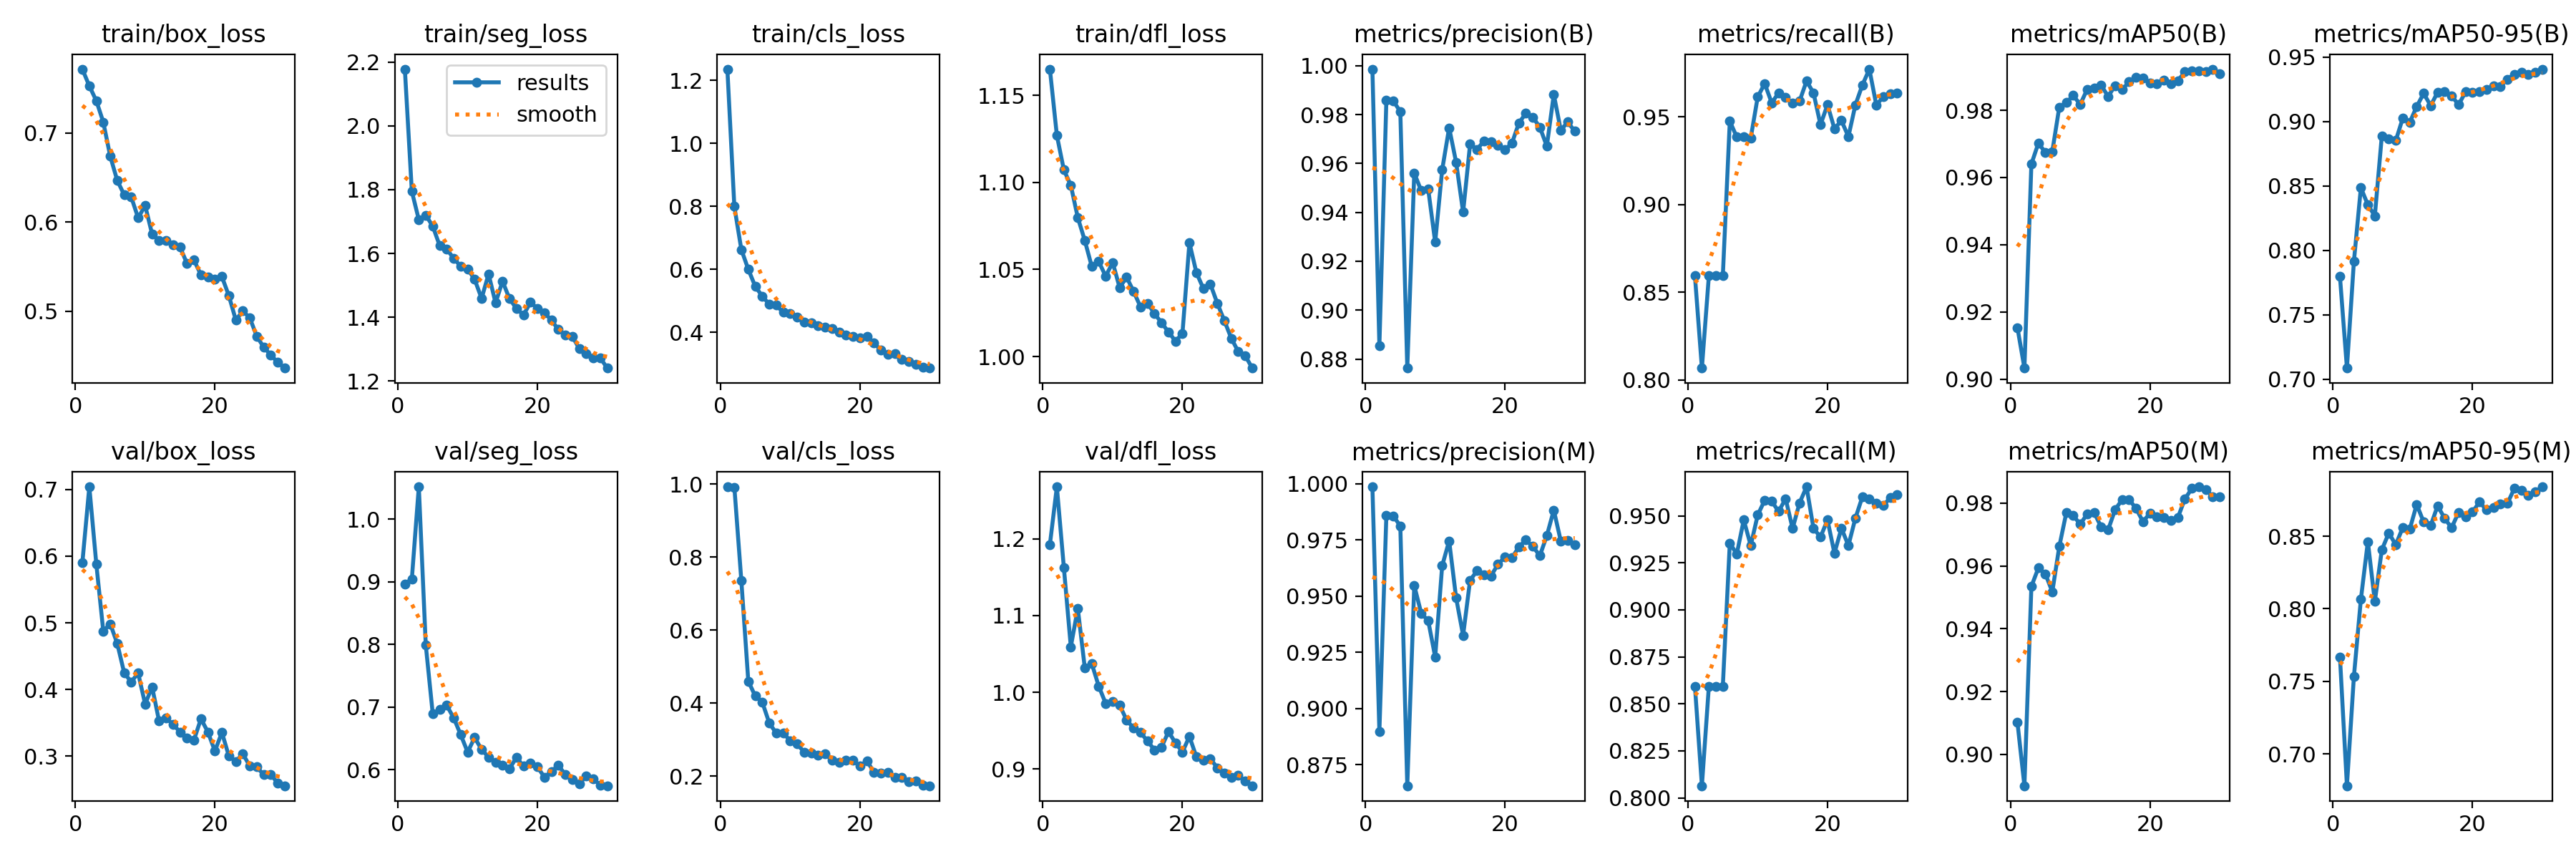
\includegraphics[width=0.98\linewidth, height=0.68\textheight, keepaspectratio]{baseline_yolov8n_640_b16_e30_results.png}
    }{
        \framebox[0.98\linewidth]{\rule{0pt}{4.5cm} results.png}
    }
\end{column}
\begin{column}{0.46\textwidth}
    \begin{block}{Chiến Lược Tối Ưu Hóa \& Hội Tụ}
    \scriptsize
    \begin{itemize}\setlength{\itemsep}{0pt}
        \item \textbf{Tối ưu:} \textbf{AdamW} (auto cho $1,410$ iter, $\beta_1=0.9$, lr $\approx 0.002$).
        \item \textbf{Lập lịch:} 3 epoch Warmup mềm, suy giảm tuyến tính (Linear Decay).
        \item \textbf{Thực nghiệm:} GPU RTX 3060 Laptop (6GB VRAM), train 30 epoch trong $16.7$ phút.
        \item Val loss giảm đều, Mask mAP@50 đạt đỉnh \textbf{0.9820}.
    \end{itemize}
    \end{block}
    \vspace{-3pt}
    \begin{alertblock}{Tại sao tắt Mosaic ở 10 Epoch cuối (\texttt{close\_mosaic=10})?}
    \scriptsize
    \begin{itemize}\setlength{\itemsep}{0pt}
        \item Mosaic ghép 4 ảnh giúp chống học vẹt ở 20 epoch đầu.
        \item 10 epoch cuối tắt Mosaic để mạng tinh chỉnh trên ảnh tự nhiên toàn vẹn.
        \item Đổi phân phối tạo \textbf{cú nảy gradient tạm thời} tại Epoch 20, sau đó loss hạ sâu hơn.
    \end{itemize}
    \end{alertblock}
\end{column}
\end{columns}
\end{frame}

% ------------------------------------------------------------------------------
% SLIDE 8: BẢNG BENCHMARK ABLATION STUDY
% ------------------------------------------------------------------------------
\begin{frame}{Đánh Giá Định Lượng: Benchmark Ablation 5 Kịch Bản (CĐR 8)}
\scriptsize
Toàn bộ 5 kịch bản thực nghiệm được huấn luyện và đo đạc thực tế trên trạm GPU \textbf{NVIDIA RTX 3060}:
\vspace{0.1cm}
\begin{table}[htbp]
\centering
\scriptsize
\renewcommand{\arraystretch}{0.95}
\begin{tabular}{l c c c c c c c c}
\toprule
\textbf{Kịch bản thực nghiệm} & \textbf{Tham số} & \textbf{FLOPs} & \textbf{Mask P} & \textbf{Mask R} & \textbf{Mask} & \textbf{Mask} & \textbf{FPS} & \textbf{VRAM} \\
 & (M) & (G) & (\%) & (\%) & \textbf{mAP@50} & \textbf{mAP@50-95} & & (GB) \\
\midrule
\rowcolor{bkblue!15} \textbf{\texttt{baseline\_yolov8n}} & \textbf{3.41} & \textbf{12.14} & \textbf{97.29} & \textbf{96.15} & \textbf{0.9820} & \textbf{0.8841} & \textbf{131.08} & \textbf{2.40} \\
\texttt{imgsz\_320}        & 3.41 & 3.04  & 96.38 & 96.67 & 0.9808 & 0.8781 & 286.18 & 0.68 \\
\texttt{batch\_8}          & 3.41 & 12.14 & 98.10 & 95.24 & 0.9843 & 0.8849 & 147.80 & 1.28 \\
\texttt{epochs\_15}        & 3.41 & 12.14 & 96.99 & 96.15 & 0.9816 & 0.8784 & 111.83 & 2.36 \\
\texttt{architecture\_yolov8s} & 11.82 & 40.34 & 97.33 & 95.46 & 0.9842 & 0.8844 & 91.20 & 4.07 \\
\bottomrule
\end{tabular}
\end{table}

\begin{alertblock}{Đánh đổi cốt lõi: Nano vs. Small}
\scriptsize
Khi nâng cấp lên \textbf{YOLOv8s-seg}, tham số tăng gấp $3.46\times$ ($11.82\,\text{M}$), FLOPs tăng $3.32\times$ ($40.34\,\text{G}$), nhưng mAP@50-95 chỉ tăng vỏn vẹn \textbf{$+0.03\%$}. Điều này khẳng định bản Nano đã trích xuất trọn vẹn đặc trưng vỏ gai sầu riêng; mở rộng mạng chỉ gây lãng phí tài nguyên tính toán!
\end{alertblock}
\end{frame}

% ------------------------------------------------------------------------------
% SLIDE 9: MA TRẬN NHẦM LẪN & KHOẢNG TIN CẬY WILSON 95%
% ------------------------------------------------------------------------------
\begin{frame}{Ma Trận Nhầm Lẫn \& Phép Tính Hậu Kỳ Khoảng Tin Cậy Wilson}
\begin{columns}[c]
\begin{column}{0.45\textwidth}
    \centering
    \IfFileExists{confusion_matrix.png}{
        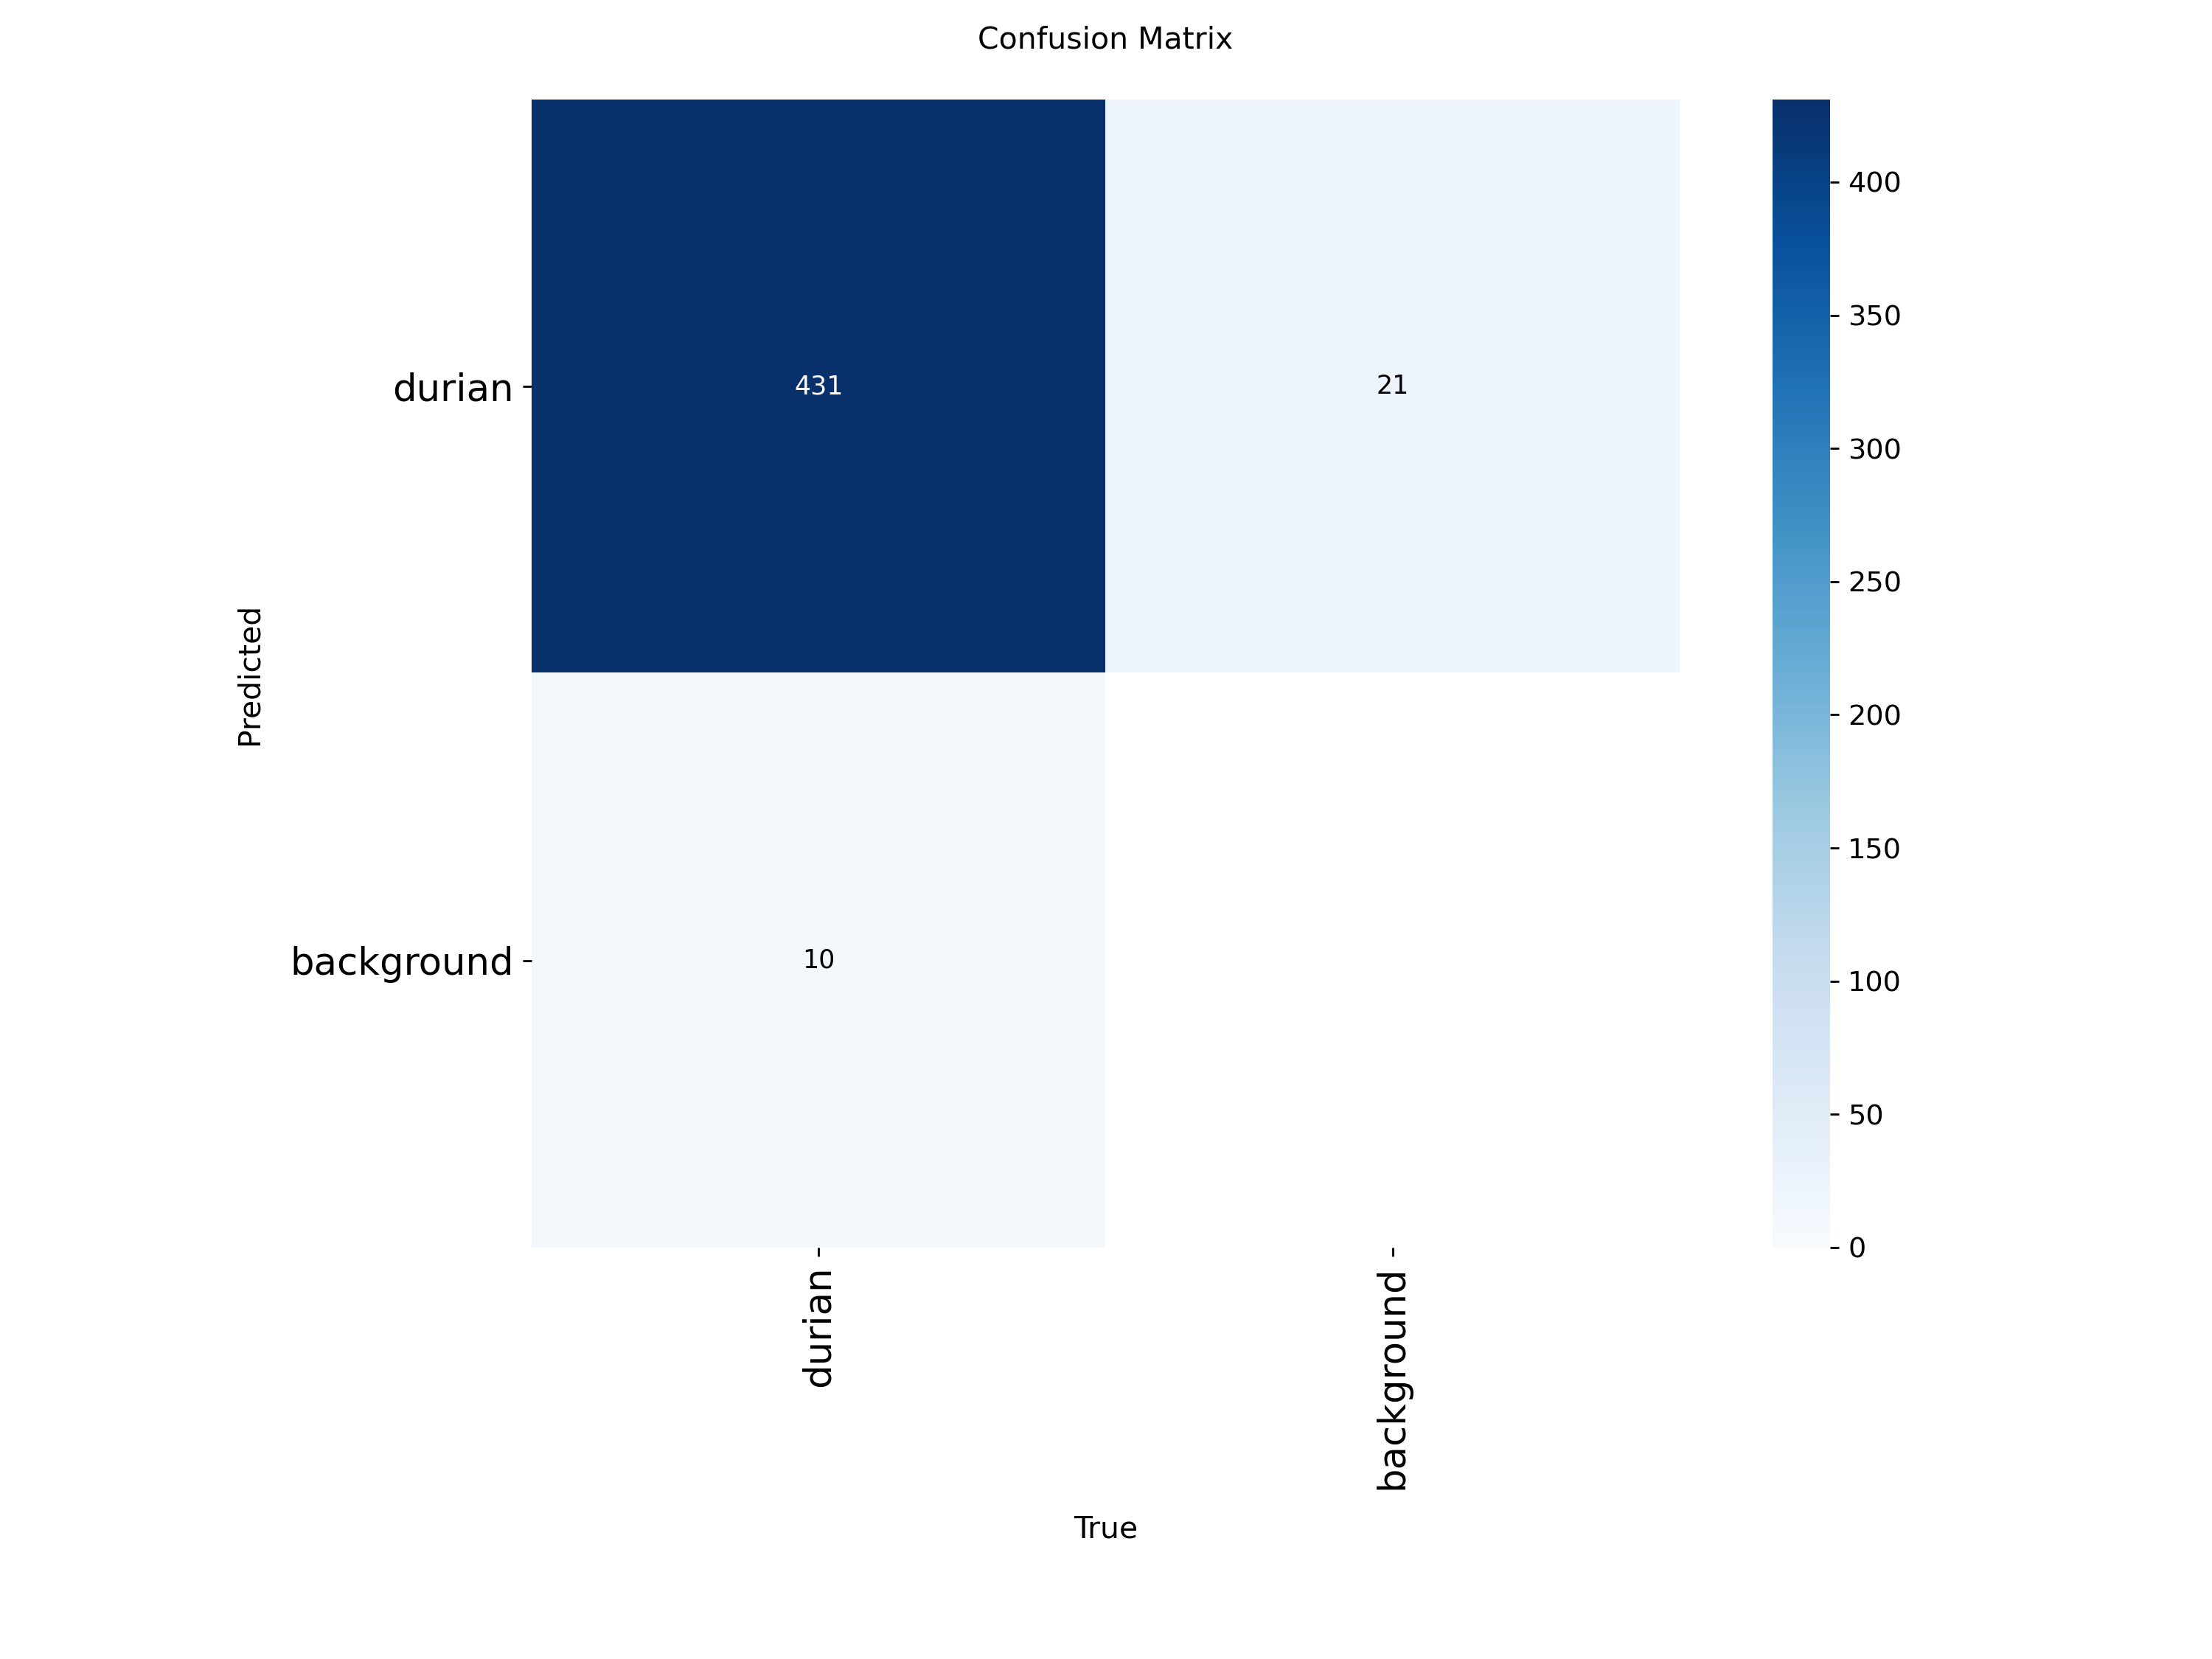
\includegraphics[width=0.92\linewidth, height=0.55\textheight, keepaspectratio]{confusion_matrix.png}
    }{
        \framebox[0.92\linewidth]{\rule{0pt}{3.5cm} confusion\_matrix.png}
    }
\end{column}
\begin{column}{0.53\textwidth}
    \begin{block}{Phân rã Ma trận Nhầm lẫn (441 Quả Ground-Truth)}
    \scriptsize
    \begin{itemize}\setlength{\itemsep}{1pt}
        \item \textbf{True Positives (TP):} \textbf{431 quả} ($97.73\%$).
        \item \textbf{False Positives (FP):} \textbf{21 ca} (nhận nhầm lá khô hoặc u thân cây).
        \item \textbf{False Negatives (FN):} \textbf{10 ca} (quả bị che khuất sâu $>85\%$).
    \end{itemize}
    \vspace{1pt}
    \centering
    $\text{Precision} = \frac{431}{452} = \mathbf{95.35\%}, \quad \text{Recall} = \frac{431}{441} = \mathbf{97.73\%}$
    \end{block}
    \vspace{-2pt}
    \begin{exampleblock}{Thống kê Hậu kỳ: Khoảng tin cậy Wilson Score 95\%}
    \scriptsize
    Tính độc lập từ $TP=431, FN=10$ ($n=441, \hat{p}=0.9773$):
    \vspace{-2pt}
    $$w = \frac{\hat{p} + \frac{z^2}{2n} \pm z \sqrt{\frac{\hat{p}(1 - \hat{p})}{n} + \frac{z^2}{4n^2}}}{1 + \frac{z^2}{n}} \implies \mathbf{[95.82\%, \; 98.78\%]}$$
    \vspace{-4pt}
    $\rightarrow$ Cận dưới xác suất $95.82\%$ bảo đảm an toàn khi robot tiếp cận.
    \end{exampleblock}
\end{column}
\end{columns}
\end{frame}

% ------------------------------------------------------------------------------
% SLIDE 10: ĐỊNH TÍNH & KHUNG GIẢI THUẬT MF-3DLOC
% ------------------------------------------------------------------------------
\begin{frame}{Kết Quả Phân Đoạn Định Tính \& Giải Thuật Định Vị MF-3DLoc}
\begin{columns}[c]
\begin{column}{0.48\textwidth}
    \centering
    \IfFileExists{baseline_yolov8n_640_b16_e30_val_batch0_pred.jpg}{
        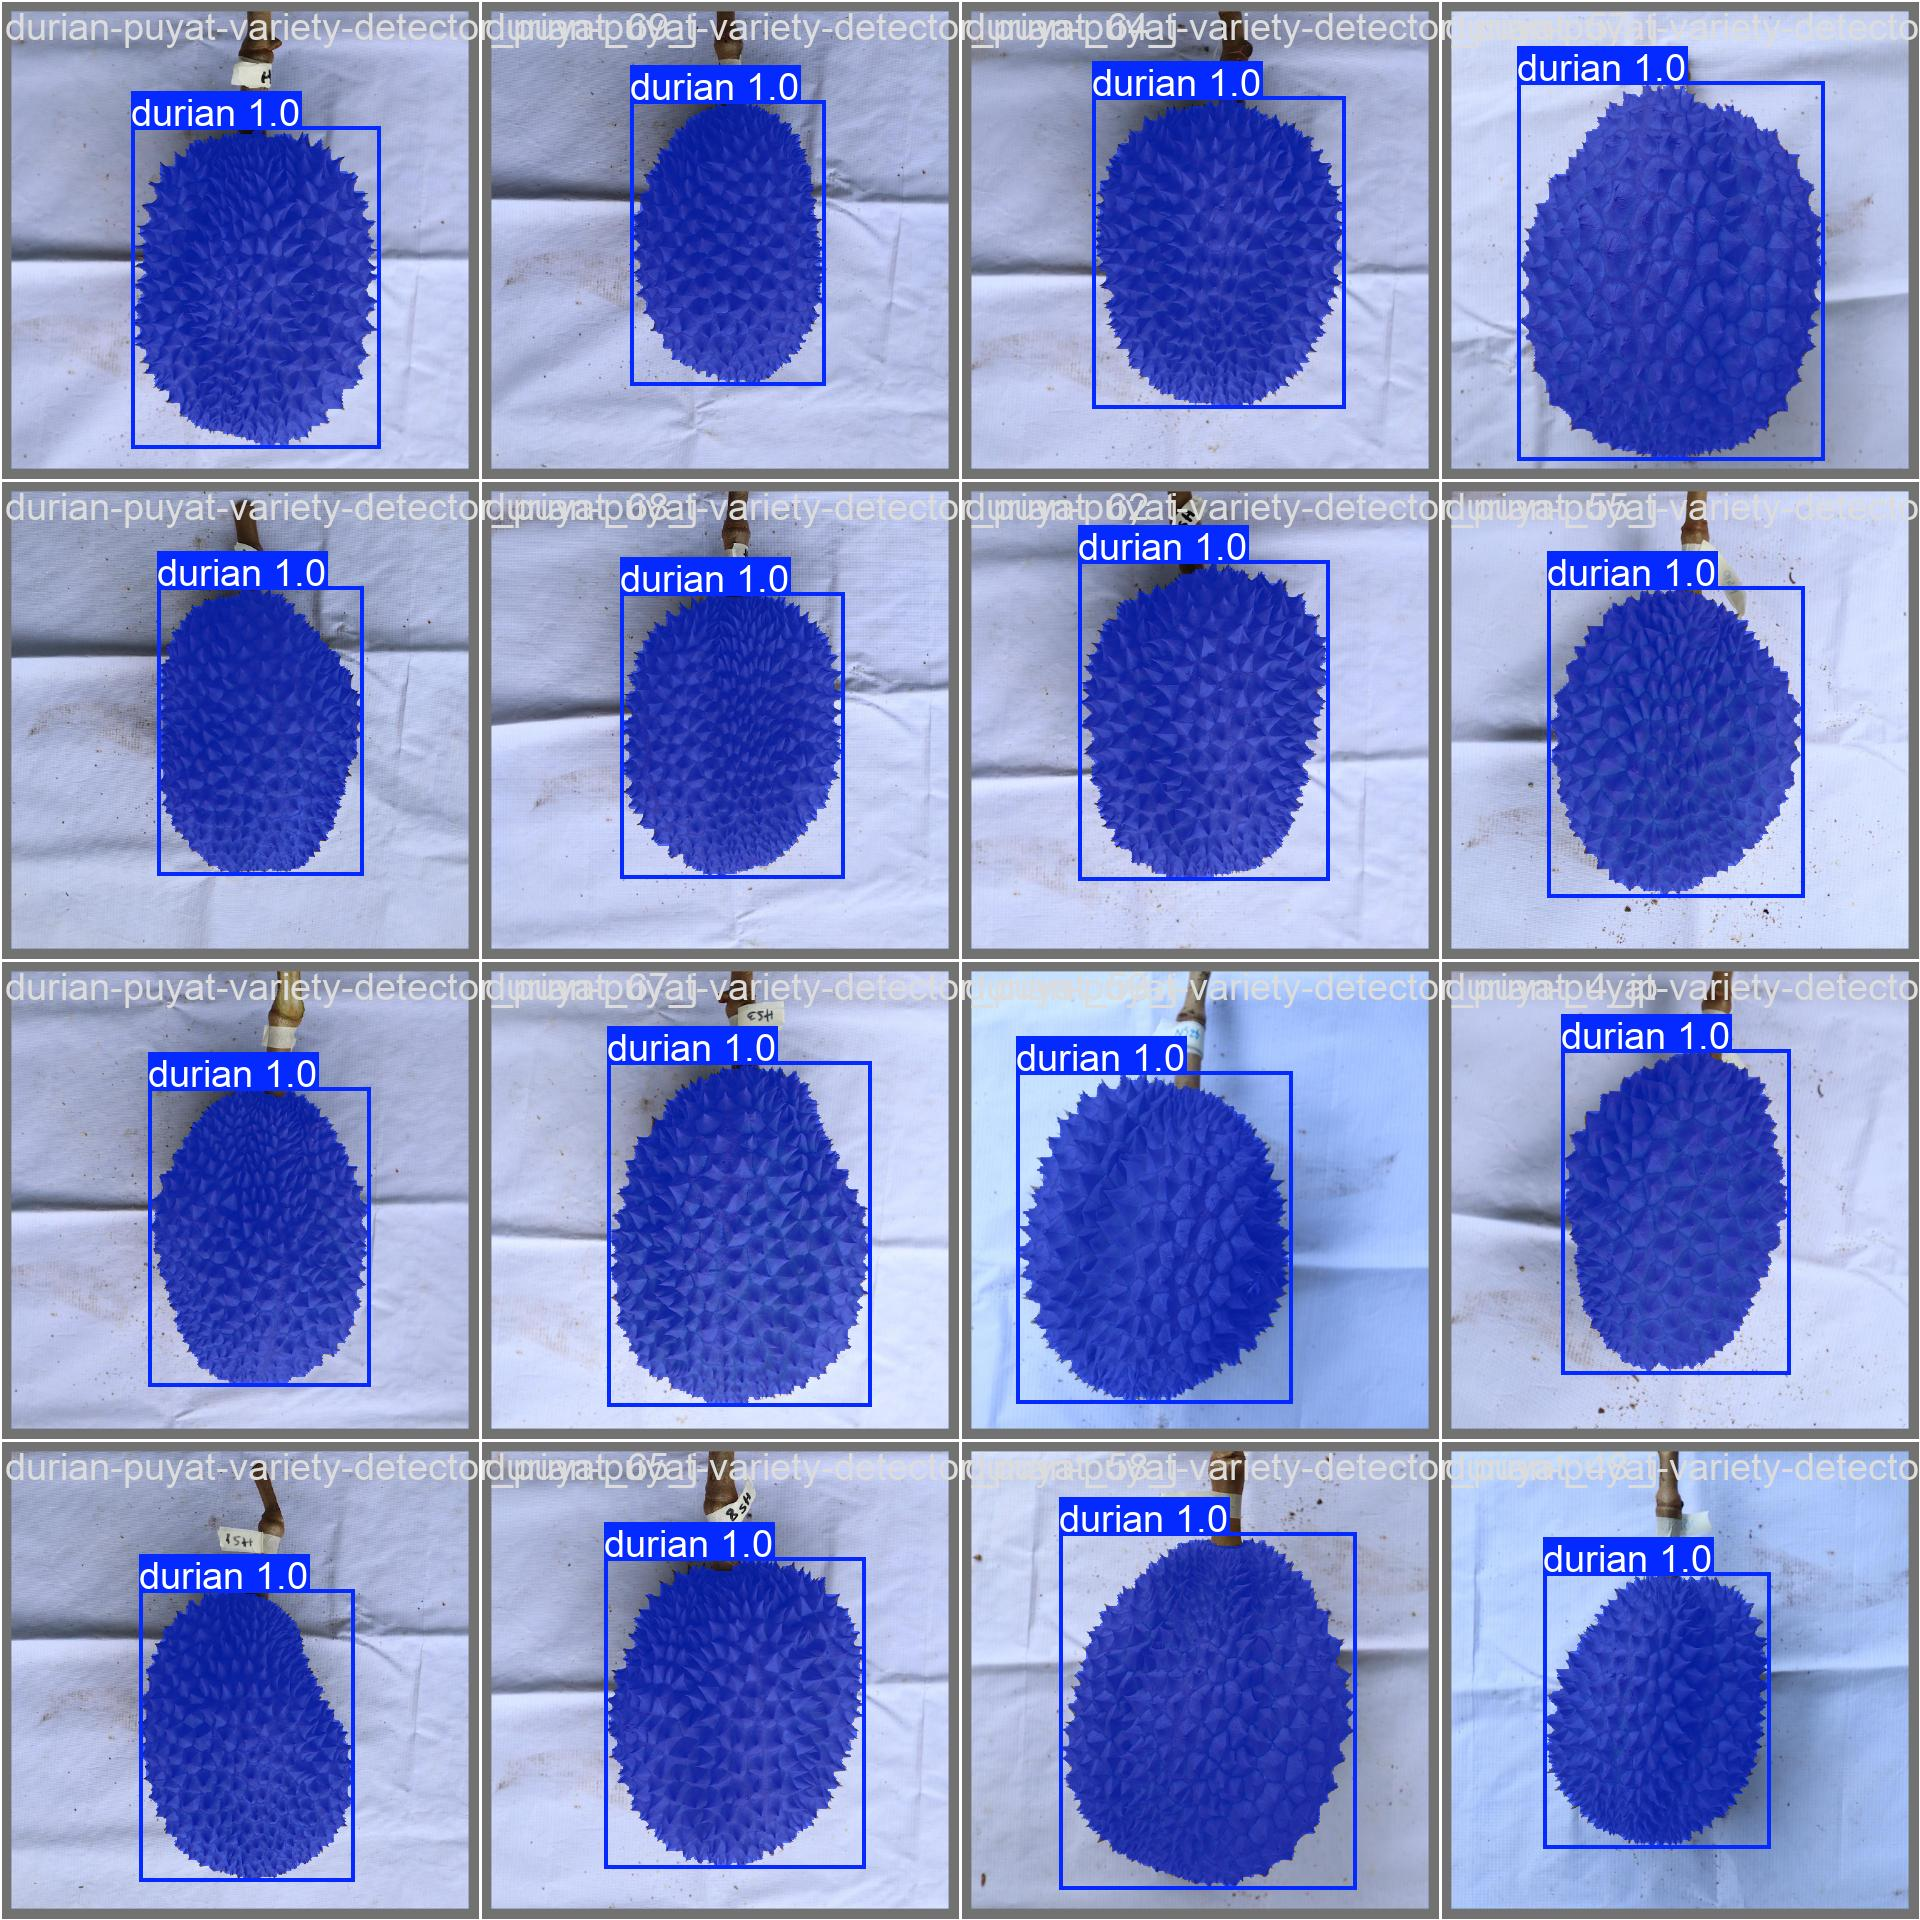
\includegraphics[width=0.95\linewidth, height=0.62\textheight, keepaspectratio]{baseline_yolov8n_640_b16_e30_val_batch0_pred.jpg}
    }{
        \framebox[0.95\linewidth]{\rule{0pt}{4.0cm} val\_batch0\_pred.jpg}
    }
    \vspace{1pt}
    \scriptsize Mặt nạ phân đoạn ôm sát viền gai từng quả trên tập validation.
\end{column}
\begin{column}{0.50\textwidth}
    \begin{block}{5 Bước của Khung Giải Thuật MF-3DLoc}
    \scriptsize
    \begin{enumerate}
        \item \textbf{Đồng bộ RGB-D:} Căn chỉnh chiều sâu về camera màu.
        \item \textbf{Trích xuất mặt nạ:} Lấy mặt nạ nhị phân $M(u, v)$ từ YOLOv8n-seg.
        \item \textbf{Lọc dải cự ly:} Giữ các điểm trong dải an toàn $[0.3\,\text{m}, 5.0\,\text{m}]$.
        \item \textbf{Ước lượng độ sâu Trung vị (Median Filter):}
        $Z = \operatorname{median}(\mathcal{D}_{\text{fruit}})$. 
        Toán tử Median có \textbf{điểm phá vỡ 50\%}, miễn nhiễm hoàn toàn với điểm nhiễu mép lá.
        \item \textbf{Chiếu ngược Pinhole:}
        $$X_C = \frac{(u_m - c_x) Z}{f_x}, \quad Y_C = \frac{(v_m - c_y) Z}{f_y}, \quad Z_C = Z$$
    \end{enumerate}
    \end{block}
\end{column}
\end{columns}
\end{frame}

% ------------------------------------------------------------------------------
% SLIDE 11: ĐO ĐẠC THỰC NGHIỆM RTX 3060 & QUY HOẠCH PHẦN CỨNG NHÚNG SPRINT 4
% ------------------------------------------------------------------------------
\begin{frame}{Đo Đạc Thực Nghiệm RTX 3060 \& Quy Hoạch Phần Cứng Nhúng Sprint 4}
\begin{columns}[T]
\begin{column}{0.48\textwidth}
    \begin{block}{Thực Đo 100\% trên GPU RTX 3060 Laptop}
    \scriptsize
    Đo đạc trực tiếp trên GPU máy trạm NVIDIA GeForce RTX 3060 Laptop (6GB VRAM, chế độ FP32):
    \begin{itemize}\setlength{\itemsep}{1pt}
        \item \textbf{Tiền xử lý (Preprocess):} $1.97\,\text{ms}$
        \item \textbf{Suy luận mạng (Inference):} $4.17\,\text{ms}$ ($\approx 240\,\text{FPS}$)
        \item \textbf{Hậu xử lý (Postprocess):} $1.49\,\text{ms}$
        \item \textbf{Tổng độ trễ toàn chu trình:} \textbf{7.63\,ms/khung hình}
        \item \textbf{Thông lượng thực tế:} \textbf{131.08\,FPS}
        \item \textbf{VRAM tiêu thụ đỉnh:} \textbf{2.40\,GB} ($40\%$ mức trần)
    \end{itemize}
    $\rightarrow$ Tốc độ đáp ứng vượt trội trên trạm điều hành.
    \end{block}
\end{column}
\begin{column}{0.50\textwidth}
    \begin{exampleblock}{Quy Hoạch Ngân Sách Cho Sprint 4 (Pi 5 16GB)}
    \scriptsize
    Phân bổ tài nguyên lý thuyết cho UGV tự hành:
    \begin{itemize}\setlength{\itemsep}{1pt}
        \item \textbf{LiDAR SLAM \& Odometry:} 1 nhân CPU, $2.0\,\text{GB}$ RAM.
        \item \textbf{ROS 2 Nav2 Planner:} 1 nhân CPU, $2.0\,\text{GB}$ RAM.
        \item \textbf{PID động học tháp pháo:} 0.5 nhân CPU, $0.5\,\text{GB}$ RAM.
        \item \textbf{Hệ điều hành \& ROS 2 DDS:} $2.0\,\text{GB}$ RAM.
        \item \textbf{Ngân sách khả dụng cho AI:} \textbf{1.5 nhân CPU, $\approx 9.5\,\text{GB}$ RAM}.
    \end{itemize}
    \textit{*Trung thực học thuật: Đo đạc thực tế trên kit Raspberry Pi 5 / Jetson là nhiệm vụ triển khai của Sprint 4.}
    \end{exampleblock}
\end{column}
\end{columns}
\end{frame}

% ------------------------------------------------------------------------------
% SLIDE 12: CA LỖI THỰC TẾ & BẢN CHẤT OVERFITTING
% ------------------------------------------------------------------------------
\begin{frame}{Phát Hiện Thực Nghiệm: Ca Lỗi Suy Biến Quy Mô \& Overfitting}
\begin{columns}[c]
\begin{column}{0.52\textwidth}
    \centering
    \IfFileExists{scale_failure_analysis.png}{
        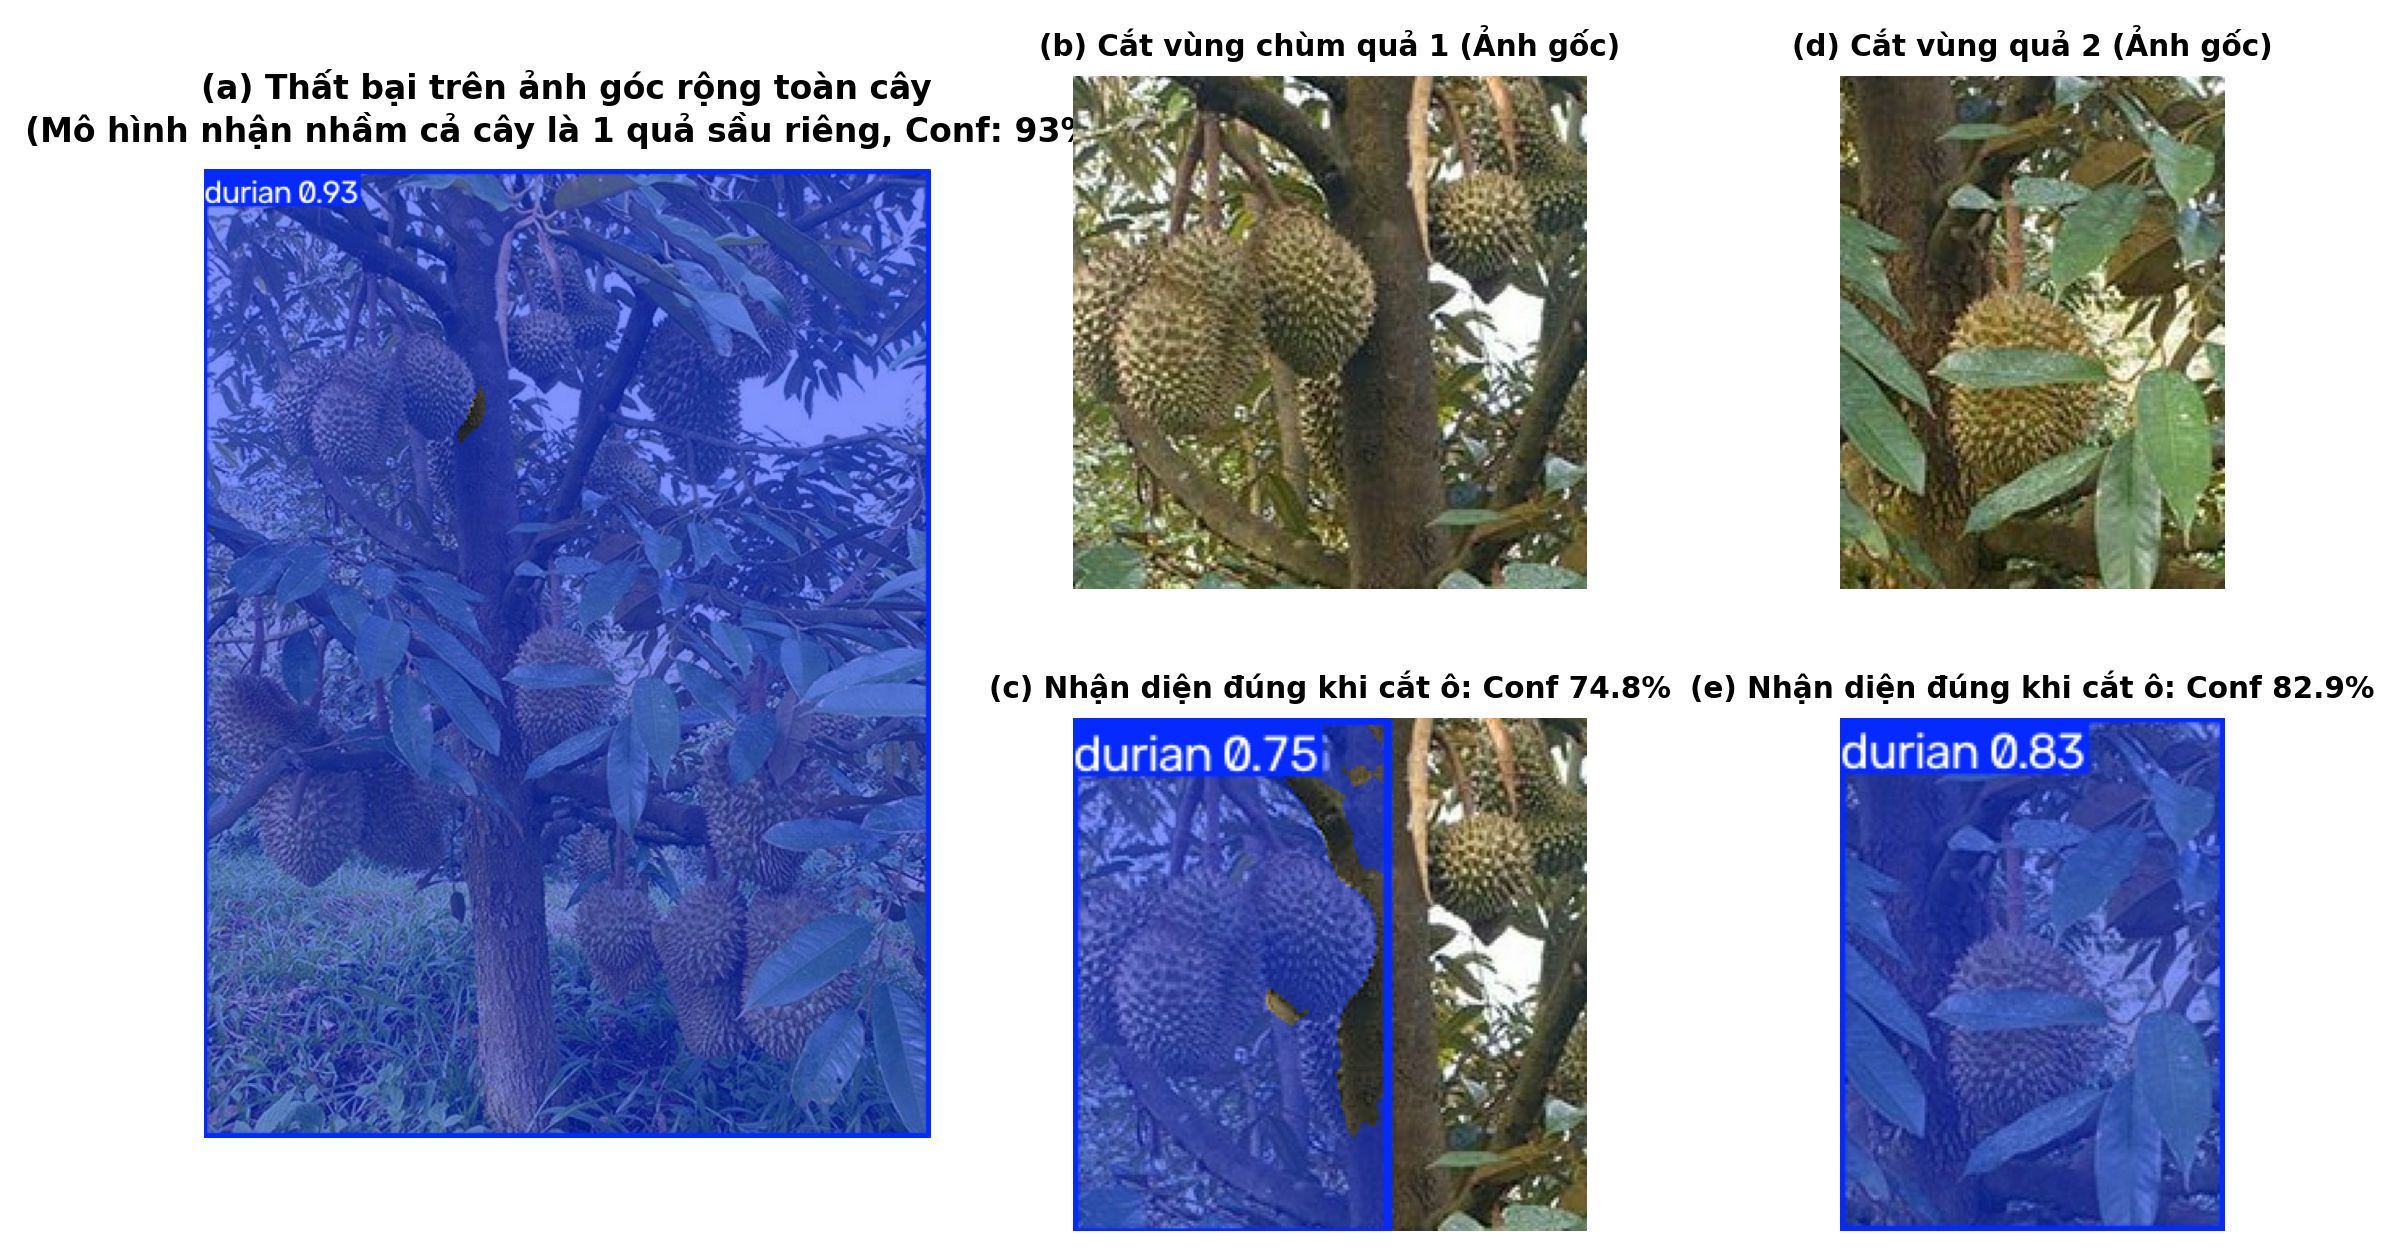
\includegraphics[width=0.98\linewidth, height=0.68\textheight, keepaspectratio]{scale_failure_analysis.png}
    }{
        \framebox[0.98\linewidth]{\rule{0pt}{4.2cm} scale\_failure\_analysis.png}
    }
\end{column}
\begin{column}{0.46\textwidth}
    \begin{alertblock}{Bóc tách 3 Dạng Sai Lệch Thực Nghiệm}
    \scriptsize
    \begin{itemize}
        \item \textbf{(a) Toàn cây góc rộng:} Nhận nhầm cả tán cây là 1 quả sầu riêng ($99.58\%$ ảnh, conf $92.56\%$).
        \item \textbf{(c) Cắt chùm quả 1:} Gộp dính 2 quả làm 1 đối tượng ($74.8\%$), bỏ sót hoàn toàn quả thứ 3 (FN)!
        \item \textbf{(e) Cắt vùng quả 2:} Bbox chiếm trọn gần $100\%$ ô cắt ($82.9\%$), mặt nạ tràn viền lên thân và lá!
    \end{itemize}
    \end{alertblock}
    \begin{block}{Kiểm toán Nguyên nhân Gốc rễ}
    \scriptsize
    \begin{itemize}
        \item \textbf{Thiên kiến quy mô:} Tập train $100\%$ ảnh chụp cận cảnh ($1.00$ quả/ảnh, chiếm $30\text{--}55\%$ diện tích).
        \item \textbf{Hội chứng chiếm trọn khung hình:} Mạng học vẹt rằng vật thể đưa vào luôn chiếm trọn ô cắt!
    \end{itemize}
    \end{block}
\end{column}
\end{columns}
\end{frame}

% ------------------------------------------------------------------------------
% SLIDE 13: THỬ NGHIỆM CHÙM QUẢ SAU-RIENG3: LỖI CHỒNG LẤN (CLUSTER OCCLUSION)
% ------------------------------------------------------------------------------
\begin{frame}{Thực Nghiệm Chùm Quả sau-rieng3: Lỗi Bỏ Sót Cá Thể Do Chồng Lấn}
\begin{columns}[c]
\begin{column}{0.47\textwidth}
    \centering
    \IfFileExists{sau-rieng3_pred.jpg}{
        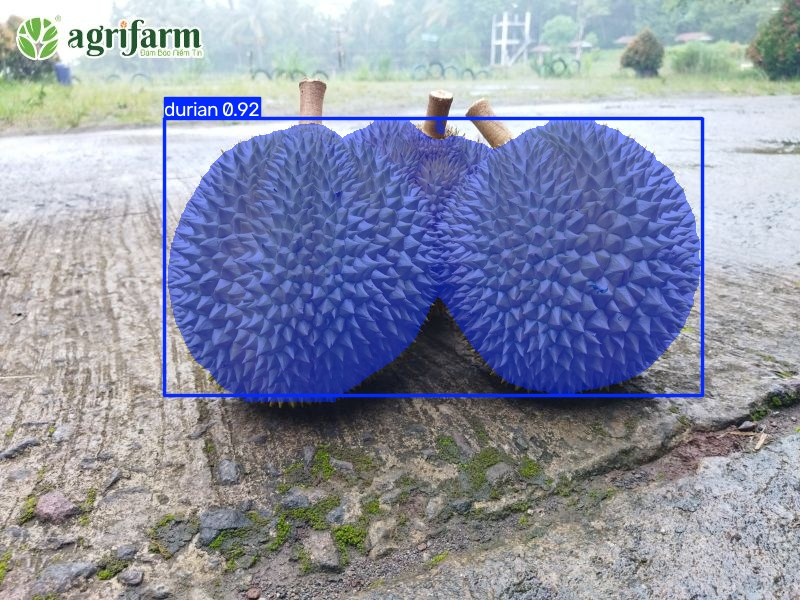
\includegraphics[width=0.98\linewidth, height=0.62\textheight, keepaspectratio]{sau-rieng3_pred.jpg}
    }{
        \framebox[0.98\linewidth]{\rule{0pt}{4.0cm} sau-rieng3\_pred.jpg}
    }
    \vspace{1pt}
    \scriptsize Thực tế có \textbf{3 quả mọc chùm đè lên nhau}, nhưng mô hình chỉ phát hiện \textbf{đúng 1 quả} (Conf $91.79\%$, BBox $31.13\%$), bỏ sót 2 quả bị che khuất!
\end{column}
\begin{column}{0.51\textwidth}
    \begin{alertblock}{Bản Chất: Cluster Occlusion \& Under-Detection}
    \scriptsize
    \begin{itemize}\setlength{\itemsep}{1pt}
        \item \textbf{Thiên lệch tập train:} Dataset Roboflow chỉ có quả đơn ($1.2$ quả/ảnh), mạng chưa từng học chùm quả đè nhau.
        \item \textbf{Đồng nhất kết cấu gai:} Vỏ gai cùng màu nâu xanh, không có viền tương phản cao để phân tách 2 quả tiếp xúc.
        \item \textbf{Triệt tiêu NMS:} Hộp bao 2 quả phía sau bị thuật toán NMS ($\text{IoU}=0.7$) loại bỏ vì trùng vị trí với quả trước.
    \end{itemize}
    \end{alertblock}
    \begin{exampleblock}{Giải Pháp Khắc Phục Cho Sprint 4}
    \scriptsize
    \begin{itemize}\setlength{\itemsep}{1pt}
        \item \textbf{Data Augmentation:} Copy-Paste ghép quả đè nhau ngẫu nhiên ($30\text{--}70\%$) và gán nhãn chuyên biệt chùm quả.
        \item \textbf{Soft-NMS / Mask-guided NMS:} Triệt tiêu dựa trên IoU mặt nạ thay vì hộp bao chữ nhật để tránh xóa nhầm.
        \item \textbf{Active Multi-view Vision:} Robot xoay camera $\pm 25^\circ$ kết hợp tách quả trên đám mây điểm 3D.
    \end{itemize}
    \end{exampleblock}
\end{column}
\end{columns}
\end{frame}

% ------------------------------------------------------------------------------
% SLIDE 13: ĐỐI CHỨNG CẮT Ô VÀ ĐỀ XUẤT GIẢI PHÁP SPRINT 4
% ------------------------------------------------------------------------------
\begin{frame}{Đối Chứng Cắt Ô \& Kế Hoạch Khắc Phục Triệt Để (Sprint 4)}
\begin{columns}[T]
\begin{column}{0.48\textwidth}
    \begin{alertblock}{Nhận định Kỹ thuật Trung thực}
    \scriptsize
    \begin{itemize}
        \item Trong Sprint 3, nhóm mới tiến hành \textbf{thử nghiệm cắt ô thủ công (manual cropping)} để kiểm chứng phản ứng của mạng.
        \item Kết quả cho thấy: Kỹ thuật cắt ô SAHI thuần túy \textbf{không thể giải quyết triệt để} nếu mạng chưa học dữ liệu tự nhiên (vì mạng vẫn nhận diện dính chùm và tràn viền thân cây).
        \item Do đó, mấu chốt bắt buộc là phải bổ sung dữ liệu thực địa ngoài vườn!
    \end{itemize}
    \end{alertblock}
\end{column}
\begin{column}{0.48\textwidth}
    \begin{exampleblock}{Định Hướng Khắc Phục Cho Sprint 4}
    \scriptsize
    \begin{enumerate}
        \item \textbf{Thu thập Dataset vườn thực địa (In-situ):} Bổ sung 300--500 ảnh toàn cây ngoài trời.
        \item \textbf{Gán nhãn tự động bằng Foundation Models:}
        \begin{itemize}
            \scriptsize
            \item Không cần vẽ tay thủ công: Dùng \textbf{Grounding DINO} \cite{liu2023grounding} (sinh BBox thô) + \textbf{SAM / SAM 2} \cite{kirillov2023segment} (tự động ôm viền gai sinh polygon mask).
            \item Con người chỉ duyệt kiểm toán nhanh.
        \end{itemize}
        \item \textbf{Tích hợp SAHI tự động \cite{akyon2022sahi}} vào ROS 2 sau khi đã fine-tune mạng.
    \end{enumerate}
    \end{exampleblock}
\end{column}
\end{columns}
\end{frame}

% ------------------------------------------------------------------------------
% SLIDE 14: THÁCH THỨC THỰC ĐỊA & BẢN QUYỀN
% ------------------------------------------------------------------------------
\begin{frame}{Khoảng Cách Triển Khai Thực Tế \& Bản Quyền Phần Mềm}
\begin{columns}[T]
\begin{column}{0.48\textwidth}
    \begin{block}{Hiện tượng Lóa Hồng Ngoại (Solar IR)}
    \scriptsize
    \begin{itemize}
        \item Nắng nhiệt đới gay gắt lấn át chùm laser IR của RealSense D453i $\rightarrow$ tạo lỗ rỗng độ sâu.
        \item \textbf{Giải pháp:} Kính lọc phân cực quang học + thuật toán nội suy chiều sâu (hole-filling) giới hạn nghiêm ngặt bên trong mặt nạ $M(u, v)$.
    \end{itemize}
    \end{block}
    \begin{block}{Rung Chấn Cơ Khí Đồi Dốc}
    \scriptsize
    \begin{itemize}
        \item Đất gồ ghề làm rung camera $\rightarrow$ mờ ảnh.
        \item \textbf{Giải pháp:} Ngàm cao su giảm chấn + bù trừ góc nghiêng qua IMU 6-DOF của D453i.
    \end{itemize}
    \end{block}
\end{column}
\begin{column}{0.48\textwidth}
    \begin{alertblock}{Giải quyết Ràng buộc Bản quyền AGPL-3.0}
    \scriptsize
    \begin{itemize}
        \item Ultralytics dính giấy phép AGPL-3.0 (buộc mở mã nguồn thương mại).
        \item \textbf{Kiến trúc cách ly thương mại:}
        \begin{enumerate}
            \scriptsize
            \item Chỉ dùng Ultralytics để train offline, sau đó xuất ra tệp trọng số chuẩn mở \textbf{ONNX}.
            \item Trên robot, viết \textbf{C++ ROS 2 Node độc lập hoàn toàn} thông qua ONNX Runtime (MIT) / NCNN (BSD), không liên kết với thư viện Python của Ultralytics.
            \item Bảo vệ $100\%$ sở hữu trí tuệ thương mại cho Doanh nghiệp.
        \end{enumerate}
    \end{itemize}
    \end{alertblock}
\end{column}
\end{columns}
\end{frame}

% ------------------------------------------------------------------------------
% SLIDE 15: KẾ HOẠCH SPRINT 4
% ------------------------------------------------------------------------------
\begin{frame}{Kế Hoạch Nhiệm Vụ Kỹ Thuật Sprint 4 (26/10 -- 08/11/2026)}
\small
Lộ trình kỹ thuật chuyển giao từ mô hình học sâu sang tích hợp robot thực địa:
\vspace{0.15cm}
\begin{table}[htbp]
\centering
\scriptsize
\renewcommand{\arraystretch}{1.1}
\begin{tabularx}{\textwidth}{c p{5.5cm} X}
\toprule
\textbf{STT} & \textbf{Nhiệm vụ kỹ thuật} & \textbf{Sản phẩm bàn giao mục tiêu} \\
\midrule
\textbf{1} & Đóng gói YOLOv8n-seg và giải thuật MF-3DLoc thành ROS 2 Node C++ độc lập trên Raspberry Pi 5. & Node C++ đọc dữ liệu RealSense D453i, chạy mô hình qua NCNN/ARM NEON, tích hợp module cắt ô SAHI. \\
\textbf{2} & Xây dựng chuỗi biến đổi tọa độ TF2 từ camera RealSense D453i sang bệ tháp pháo UGV. & Xuất bản topic \texttt{/turret/target\_3d\_goal} chứa vectơ metric $(X_T, Y_T, Z_T)$ điều khiển góc quay pan-tilt. \\
\textbf{3} & Kiểm chứng độ chính xác ngắm bắn vòng kín trong mô phỏng Gazebo độ trung thực cao. & Biểu đồ và video Gazebo đánh giá sai số ngắm bắn dưới tác động của rung chấn xe UGV trên sườn đồi. \\
\bottomrule
\end{tabularx}
\end{table}
\end{frame}

% ------------------------------------------------------------------------------
% SLIDE 16: TÀI LIỆU THAM KHẢO
% ------------------------------------------------------------------------------
\begin{frame}[allowframebreaks]{Tài Liệu Tham Khảo Chọn Lọc}
\scriptsize
\begin{thebibliography}{10}
\bibitem{fu2020rgbd}
L.~Fu et al., ``Application of consumer RGB-D cameras for fruit detection and localization in field: A critical review,'' \textit{Comput. Electron. Agric.}, tập~177, tr. 105687, 2020.

\bibitem{lin2021fruit}
G.~Lin et al., ``Three-dimensional reconstruction of fruits and branches using instance segmentation and geometry analysis,'' \textit{Comput. Electron. Agric.}, tập~184, tr. 106107, 2021.

\bibitem{kang2020dasnet}
H.~Kang và C.~Chen, ``Fruit detection, segmentation and 3D visualisation of environments in apple orchards,'' \textit{Comput. Electron. Agric.}, tập~171, tr. 105302, 2020.

\bibitem{akyon2022sahi}
F.~C.~Akyon et al., ``Slicing Aided Hyper Inference and fine-tuning for small object detection,'' trong \textit{IEEE ICIP}, 2022, tr. 966--970.

\bibitem{zheng2020ciou}
Z.~Zheng et al., ``Distance-IoU loss: Faster and better learning for bounding box regression,'' trong \textit{AAAI}, 2020, tr. 12\,993--13\,000.

\bibitem{li2020generalized}
X.~Li et al., ``Generalized focal loss: Learning qualified and distributed bounding boxes for dense object detection,'' trong \textit{NeurIPS}, 2020.

\bibitem{wilson1927probable}
E.~B.~Wilson, ``Probable inference, the law of succession, and statistical inference,'' \textit{J. Amer. Statist. Assoc.}, 1927.

\bibitem{kirillov2023segment}
A.~Kirillov et al., ``Segment Anything,'' trong \textit{IEEE/CVF ICCV}, 2023.

\bibitem{liu2023grounding}
S.~Liu et al., ``Grounding DINO: Marrying DINO with Grounded Pre-Training,'' trong \textit{ECCV}, 2024.
\end{thebibliography}
\end{frame}

% ------------------------------------------------------------------------------
% SLIDE 17: PHẦN KẾT VÀ HỎI ĐÁP (Q&A)
% ------------------------------------------------------------------------------
\begin{frame}
\centering
\vspace{1.0cm}
{\Huge\bfseries\color{bkblue} XIN CHÂN THÀNH CẢM ƠN!}\\[0.4cm]

\begin{beamercolorbox}[sep=8pt,center,rounded=true,shadow=true]{palette primary}
    \textbf{CO3133: Học sâu và Ứng dụng -- Báo cáo Tiến độ 3 (Sprint 3)}\\
    \textit{Nhóm sinh viên: Trần Hữu Hoàng Long \& Trương Gia Hy}
\end{beamercolorbox}
\end{frame}

\end{document}
